\section{Prototype et résultats}

\subsection{État livré}

Le prototype réunit la boîte, le plateau motorisé, le laser, les deux
caméras, le PCB de commande, le capteur de capot, l'écran tactile et
l'interface web. Le pipeline réel produit des nuages PLY intermédiaires et un
maillage STL.

\begin{figure}[H]
  \centering
  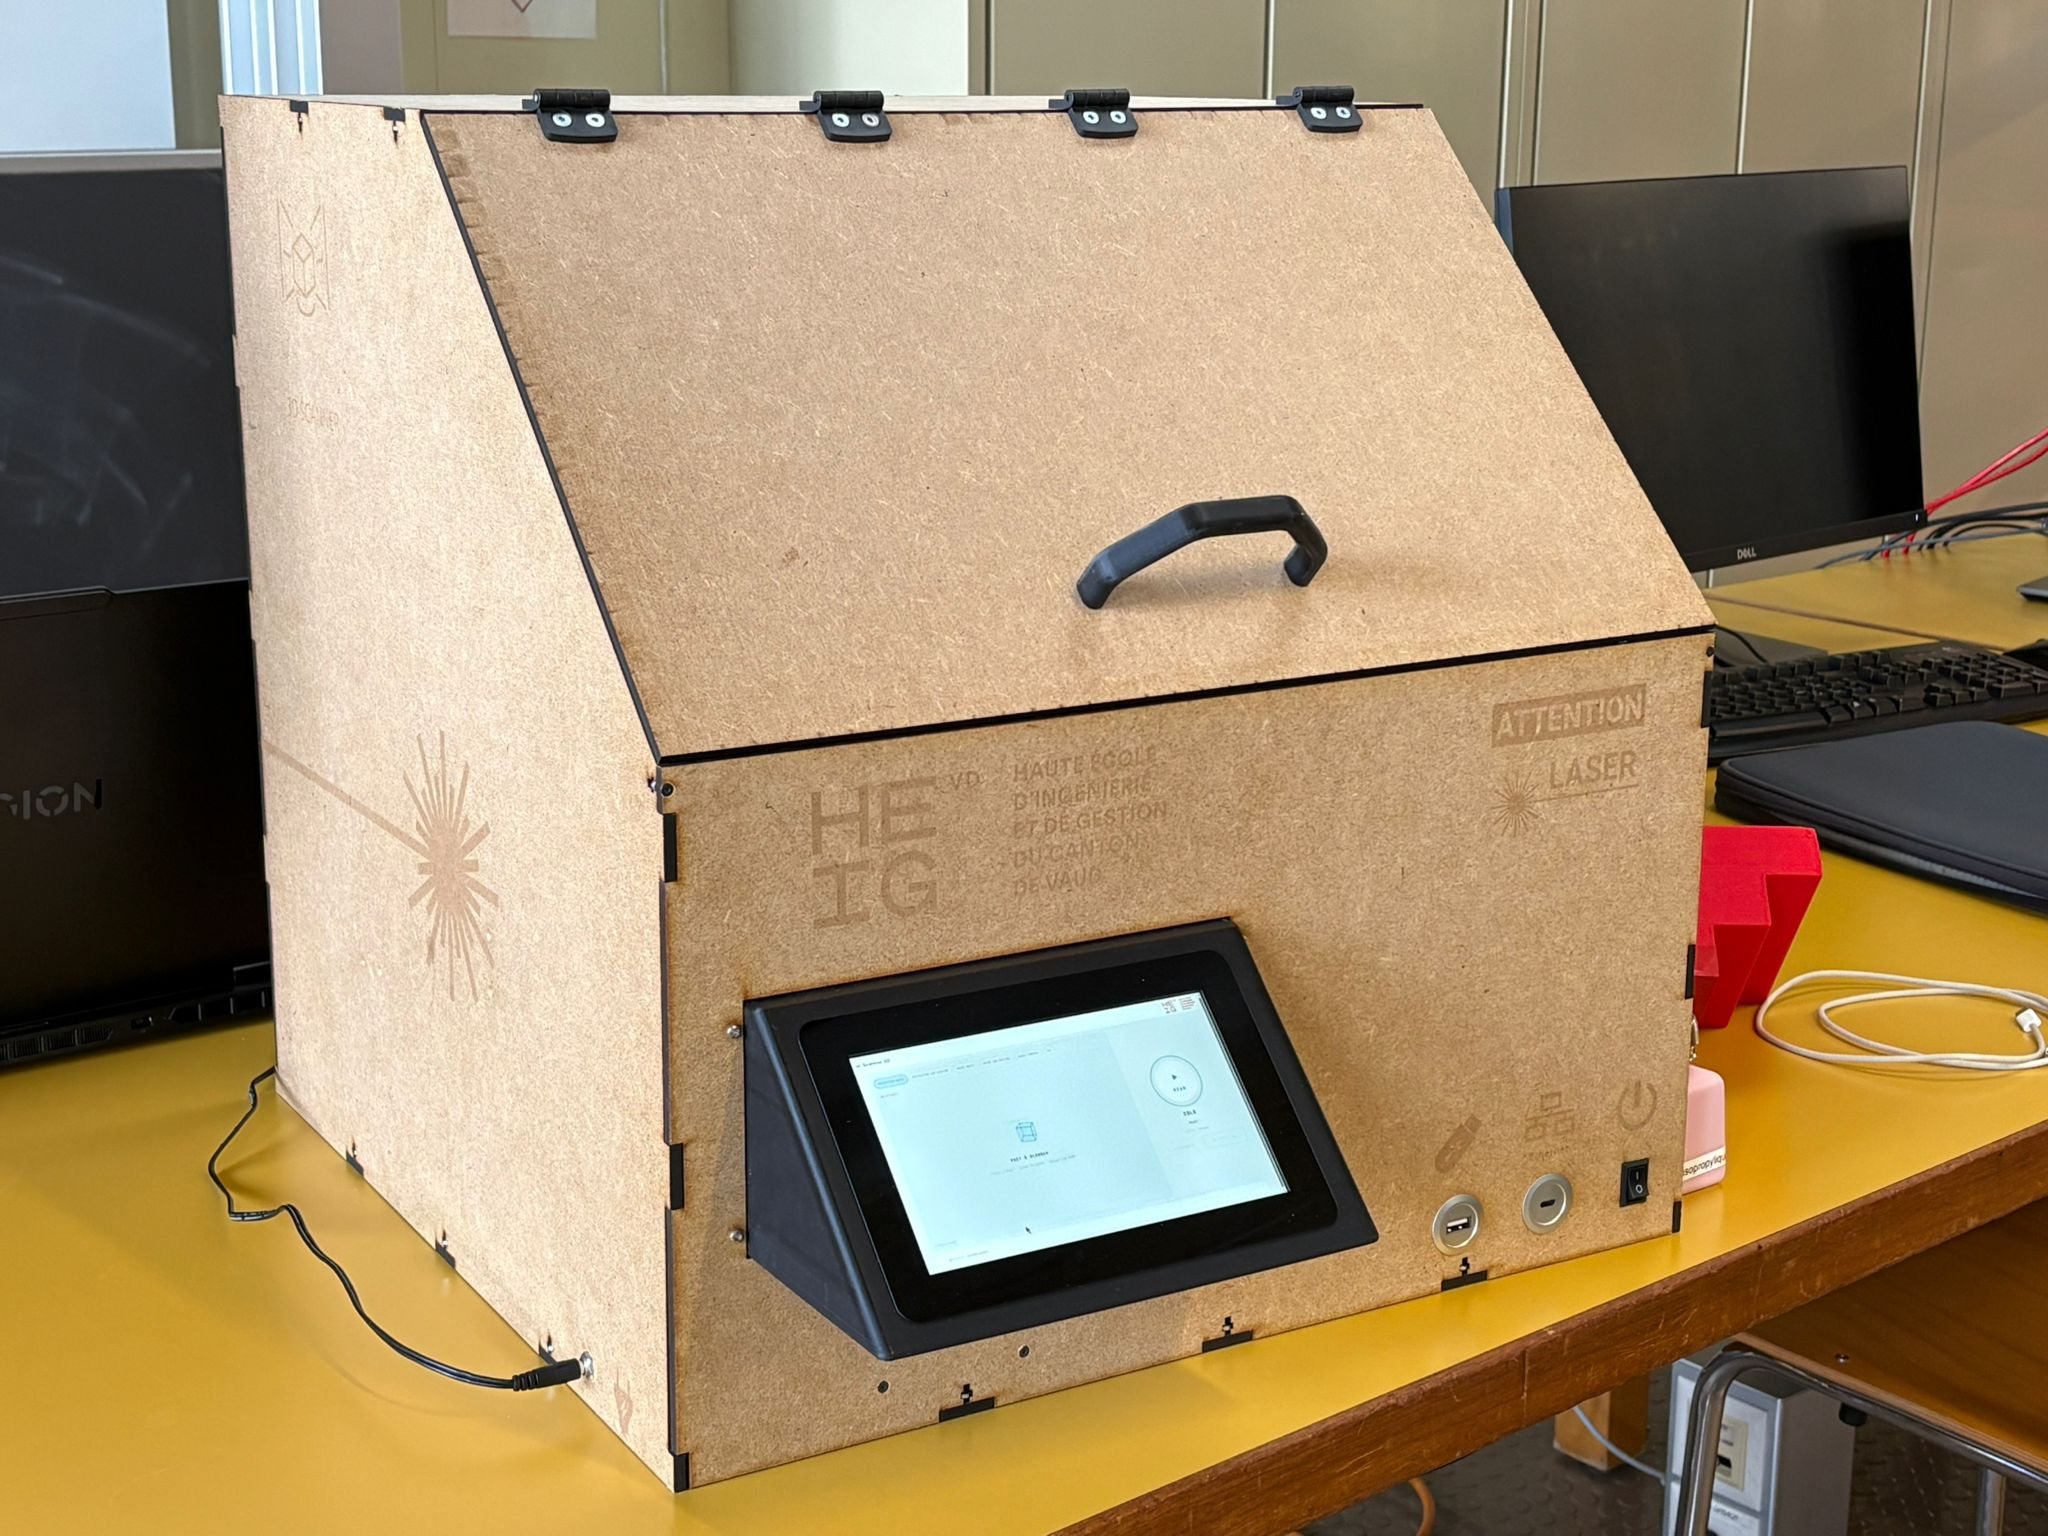
\includegraphics[width=0.6\linewidth]{images/boite_finale.jpeg}
  \caption{Vue extérieure du prototype final assemblé.}
  \label{fig:boite-finale}
\end{figure}

\begin{table}[H]
  \centering
  \small
  \begin{tabular}{@{}p{4.1cm}p{3cm}p{7cm}@{}}
    \toprule
    \textbf{Fonction} & \textbf{Statut} & \textbf{Justification} \\
    \midrule
    Acquisition à deux caméras & Démontrée & Pipeline matériel et captures par position. \\
    Interlock et arrêt laser & Testés & Capteur monté, contrôles avant activation et surveillance périodique à 100~ms. \\
    Extraction et triangulation & Démontrées & Nuages PLY produits par caméra. \\
    Fusion et maillage & Démontrés & Export Poisson STL disponible. \\
    Interface et export USB & Démontrés & Routes web, viewer et copie USB implémentés. \\
    \bottomrule
  \end{tabular}
  \caption{État des fonctions et validations.}
  \label{tab:maturite}
\end{table}

\subsection{Résultats}
\label{sec:prototype-resultats}

Un cycle complet, depuis le lancement jusqu'à l'export, a été chronométré à
environ 8 minutes. L'objectif O3 est donc atteint pour la configuration testée.
Les deux points de vue récupèrent davantage de zones sur les formes anguleuses
qu'une acquisition mono-caméra.

\begin{figure}[H]
  \centering
  \begin{minipage}{0.45\linewidth}
    \centering
    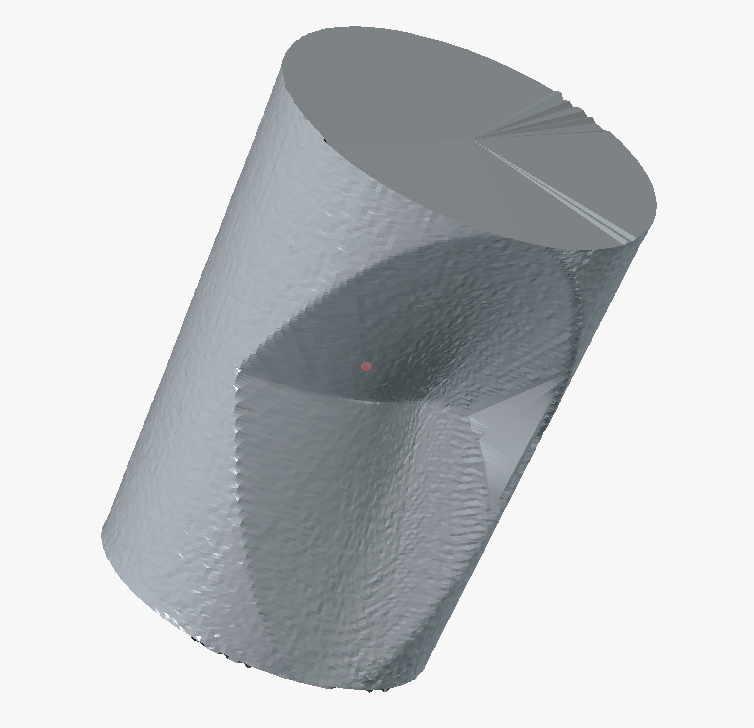
\includegraphics[width=0.85\linewidth]{images/screen_cylindre_stl.png}
    \\\small (a) Maillage d'un cylindre.
  \end{minipage}\hfill
  \begin{minipage}{0.45\linewidth}
    \centering
    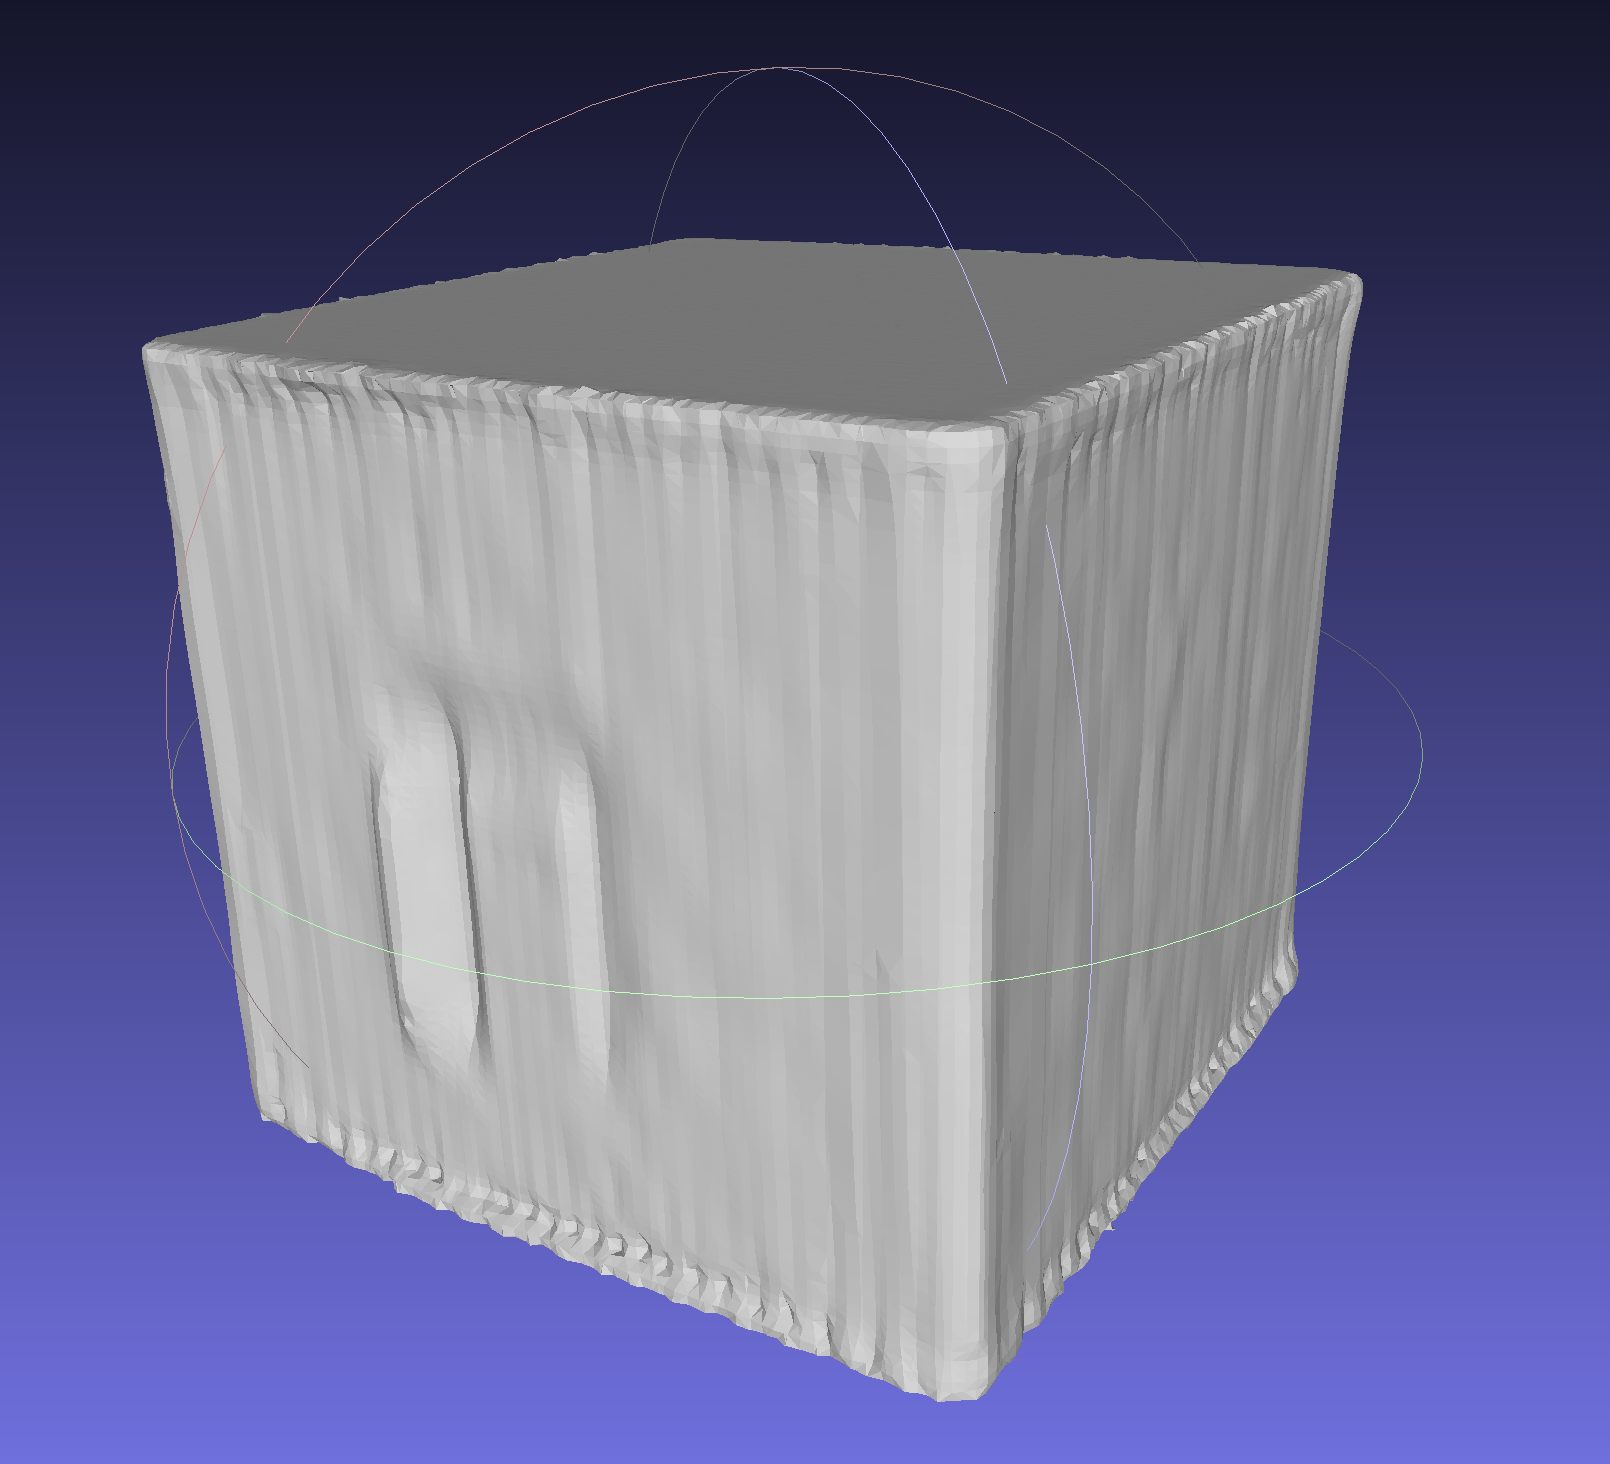
\includegraphics[width=0.85\linewidth]{images/cube_double_camera.png}
    \\\small (b) Résultat à deux caméras sur un cube.
  \end{minipage}
  \caption{Exemples de reconstructions produits par le pipeline final.}
  \label{fig:resultats-scans}
\end{figure}

\begin{figure}[H]
  \centering
  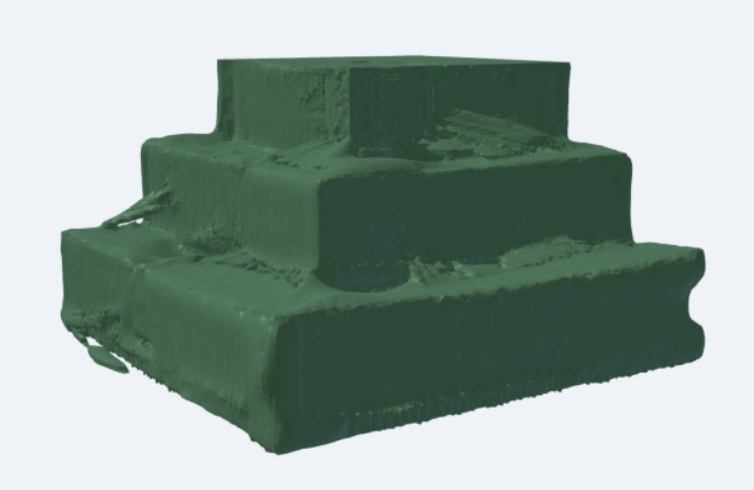
\includegraphics[width=0.68\linewidth]{images/resultat_escalier.png}
  \caption{Maillage obtenu pour la pièce en escalier. Les différents niveaux
  sont reconnaissables; des irrégularités restent visibles près des arêtes et
  dans certaines zones moins bien observées.}
  \label{fig:resultat-escalier}
\end{figure}

Les comparaisons dimensionnelles réalisées sur les pièces reconstruites
montrent une précision satisfaisante dans le plan horizontal: les dimensions
relevées suivant les axes $X$ et $Y$ restent généralement dans un intervalle
d'environ $\pm 2$\,mm par rapport aux dimensions de référence. L'échelle
verticale est en revanche moins fidèle et présente des écarts plus importants
sur l'axe $Z$. Cette différence semble liée à la plus forte sensibilité de la
hauteur reconstruite à l'ensemble de la chaîne géométrique, notamment au
réglage des poses, au plan laser et à la visibilité des surfaces horizontales.
Les essais disponibles ne permettent toutefois pas d'isoler une cause unique.
Le scanner restitue donc correctement la forme générale et les dimensions
dans le plan, tandis que la mesure suivant $Z$ demande encore une calibration
plus approfondie avant de pouvoir être considérée comme métrologique.

\begin{table}[H]
  \centering
  \begin{tabular}{@{}p{6cm}p{4cm}p{3.5cm}@{}}
    \toprule
    \textbf{Indicateur} & \textbf{Résultat} & \textbf{Cible} \\
    \midrule
    Cycle complet & $\approx$\,8\,min & $\leq 10$\,min \\
    Export STL & Produit & Obligatoire \\
    Coût réellement engagé & 133,83\,CHF & $\leq 300$\,CHF \\
    Dimensions extérieures & $500\times500\times500$\,mm & $\leq 500^3$\,mm \\
    \bottomrule
  \end{tabular}
  \caption{Résultats disponibles à la livraison.}
  \label{tab:perf-attendues}
\end{table}

\subsection{Limites}

La qualité dépend du réglage optique, des masques et de l'ajustement
extrinsèque. Les surfaces brillantes, très sombres, vertes ou cachées peuvent
dégrader l'extraction.

L'amélioration de la précision suivant l'axe $Z$ constitue un axe prioritaire
pour la suite du projet. Un travail complémentaire devra chercher à identifier
l'origine des écarts observés, en étudiant notamment la calibration du plan
laser, les poses extrinsèques des caméras et la propagation des erreurs dans la
triangulation. Une campagne de mesures sur plusieurs pièces étalons permettrait
ensuite de quantifier séparément la précision et la répétabilité sur les trois
axes.

Un mode de scan utilisant uniquement la caméra supérieure pourrait également
être avantageux pour les pièces simples et entièrement visibles depuis ce
point de vue. Il éviterait alors le regroupement de deux nuages et réduirait la
sensibilité du résultat aux extrinsèques relatives des caméras. L'acquisition
à deux caméras resterait toutefois essentielle pour les pièces plus complexes,
présentant des faces masquées ou des zones insuffisamment observées par une
seule caméra. Une évolution de l'interface pourrait ainsi permettre de choisir
le mode d'acquisition selon la géométrie de la pièce.
